% !TEX root = ../../../thesis.tex
%TODO: fix values.
In order to make SNS junctions we first sputtered \qty{1}{\nano\meter} of \ce{Cu} on our \ce{SiO} wafer, on top of this we added our \qty{1}{\nano\meter} of \ce{Nb} and capped it with \qty{7}{\nano\meter} of \ce{Au}. We again used the FIB to create the fine structures, see Figure~\ref{fig:CP2.6B-SEM-images}.

\begin{figure}[ht]
	\begin{subfigure}[t]{0.3\textwidth}
		\centering
		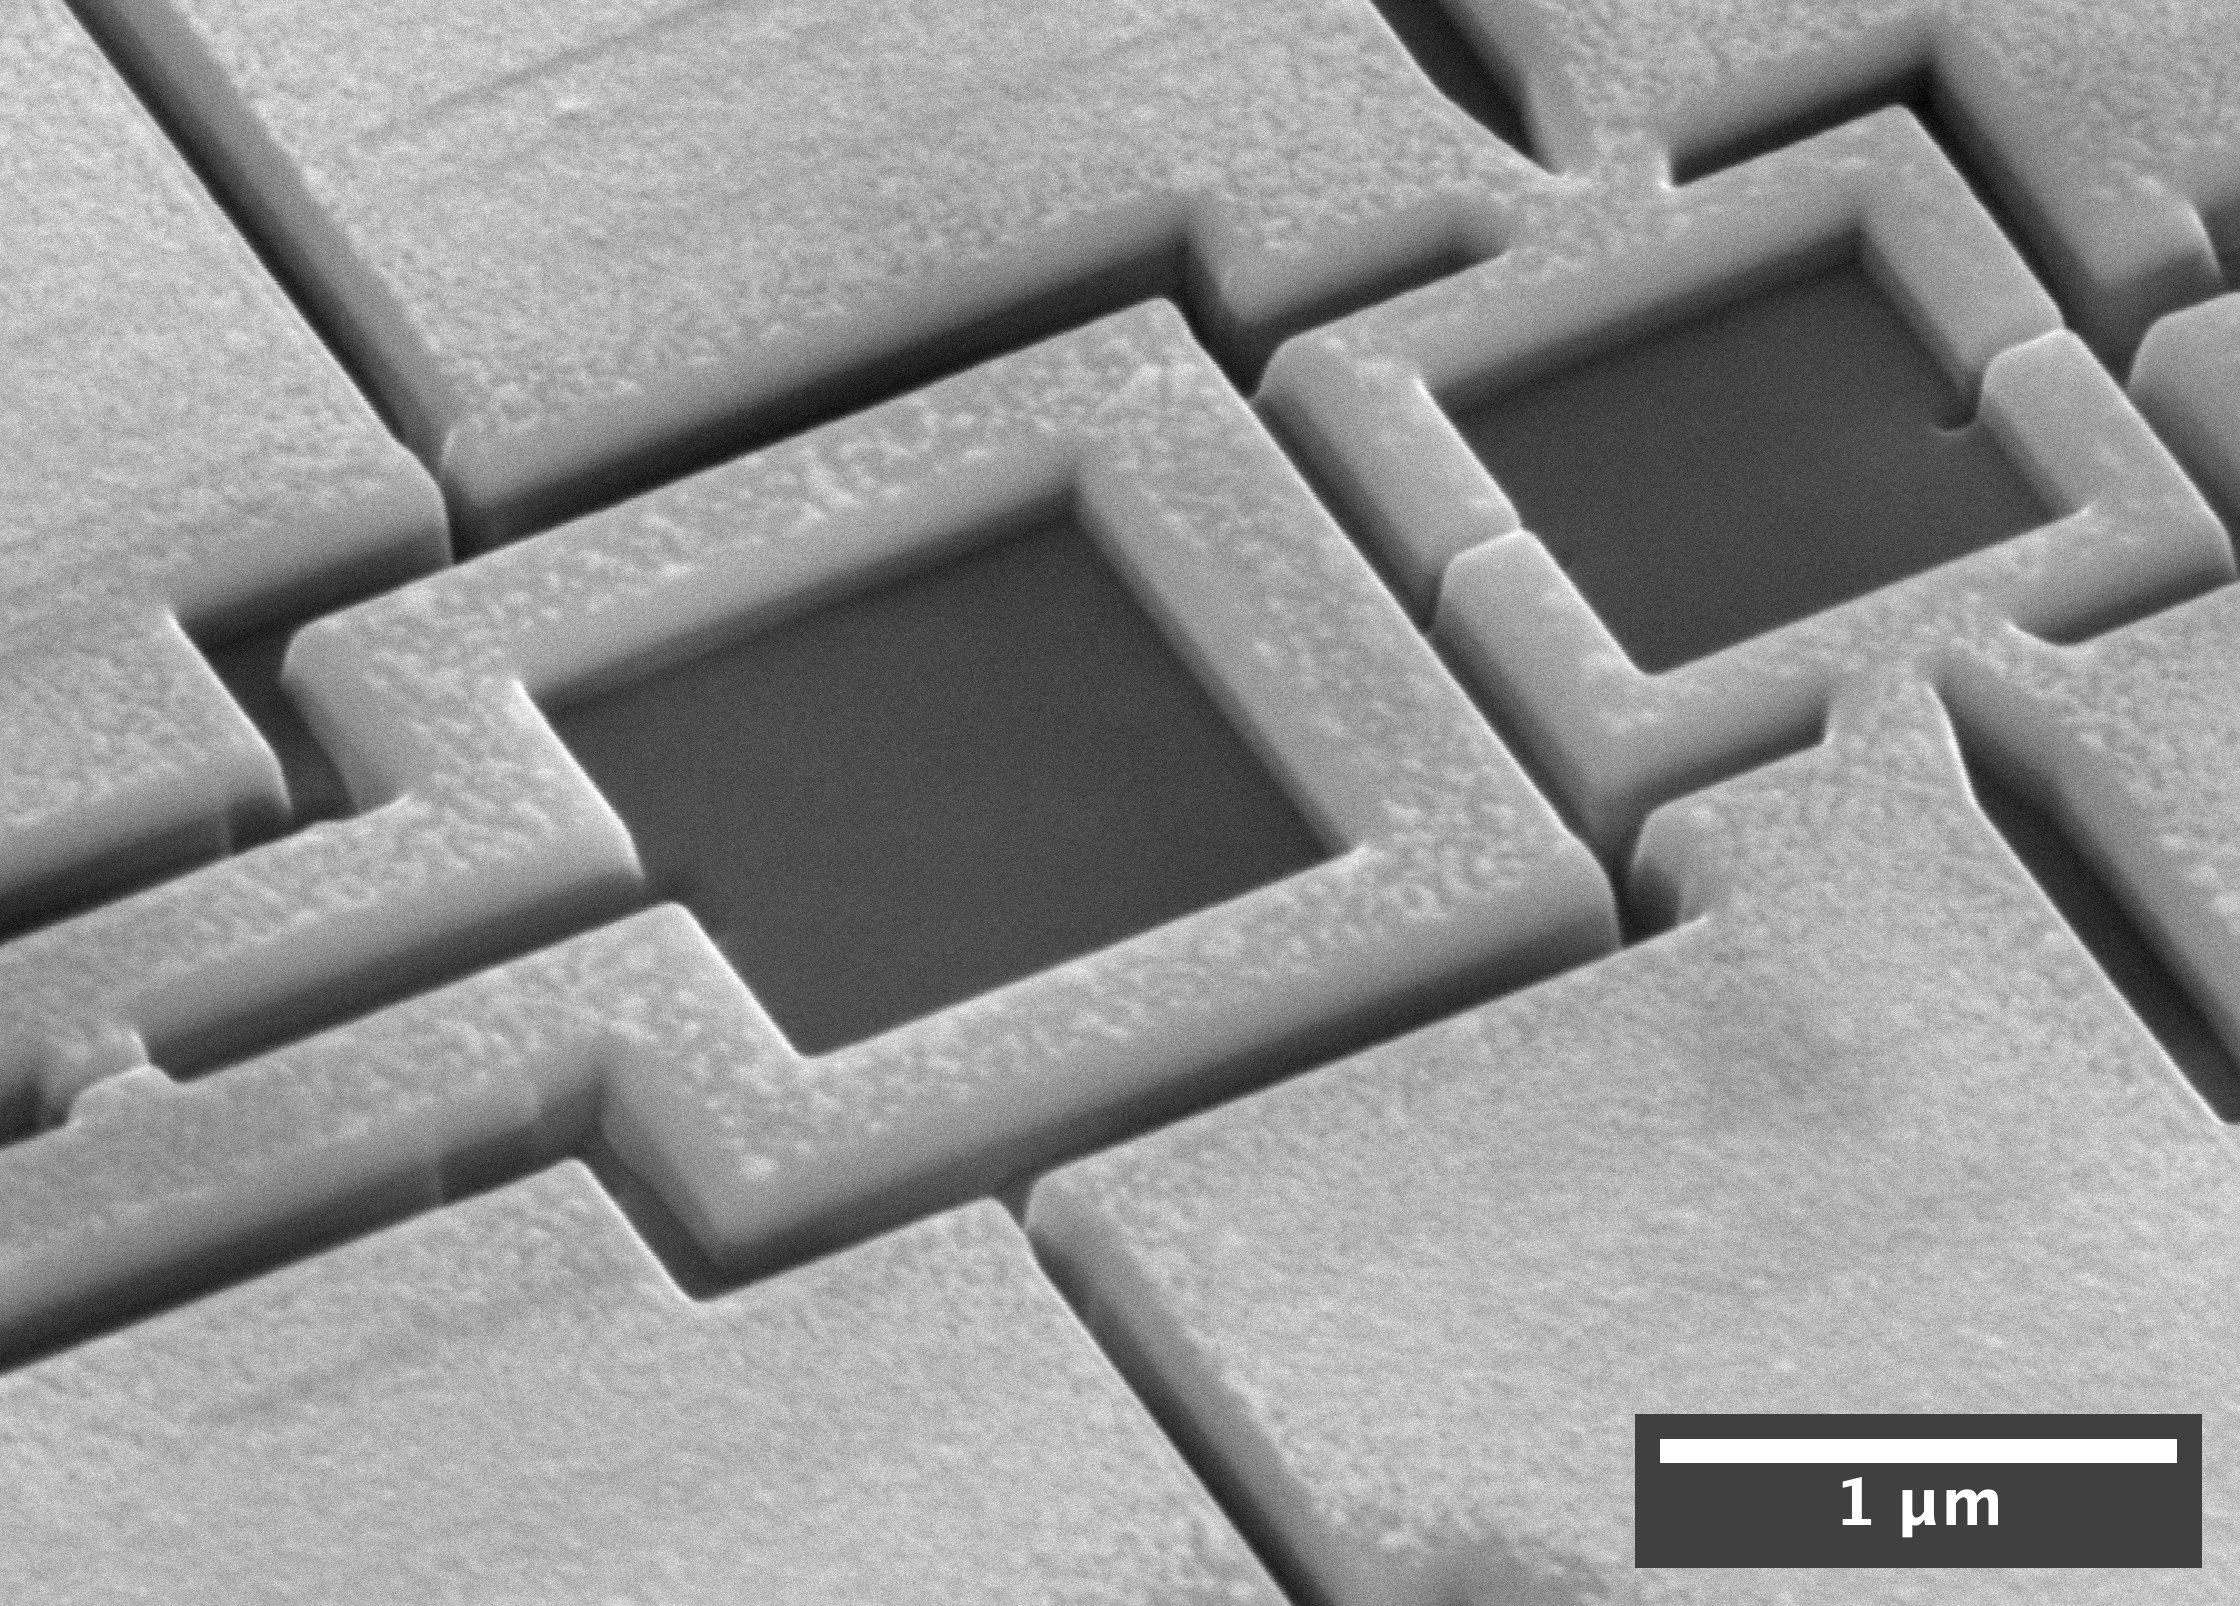
\includegraphics[width=\textwidth]{figures/samples/CP2/CP2.6B_SEM_overview.jpg}
		\subcaption{Overview of the device. The top loop shows the dc-SQUID and the bottom is the junction loop. In-between the arms extending down from the junction loop is the actual Josephson junction under study. The inner and outer diameter of the junction loop are \qty{1.3}{\micro\meter} and \qty{2}{\micro\meter} respectively.}
	\end{subfigure}
	\hfill
	\begin{subfigure}[t]{0.3\textwidth}
		\centering
		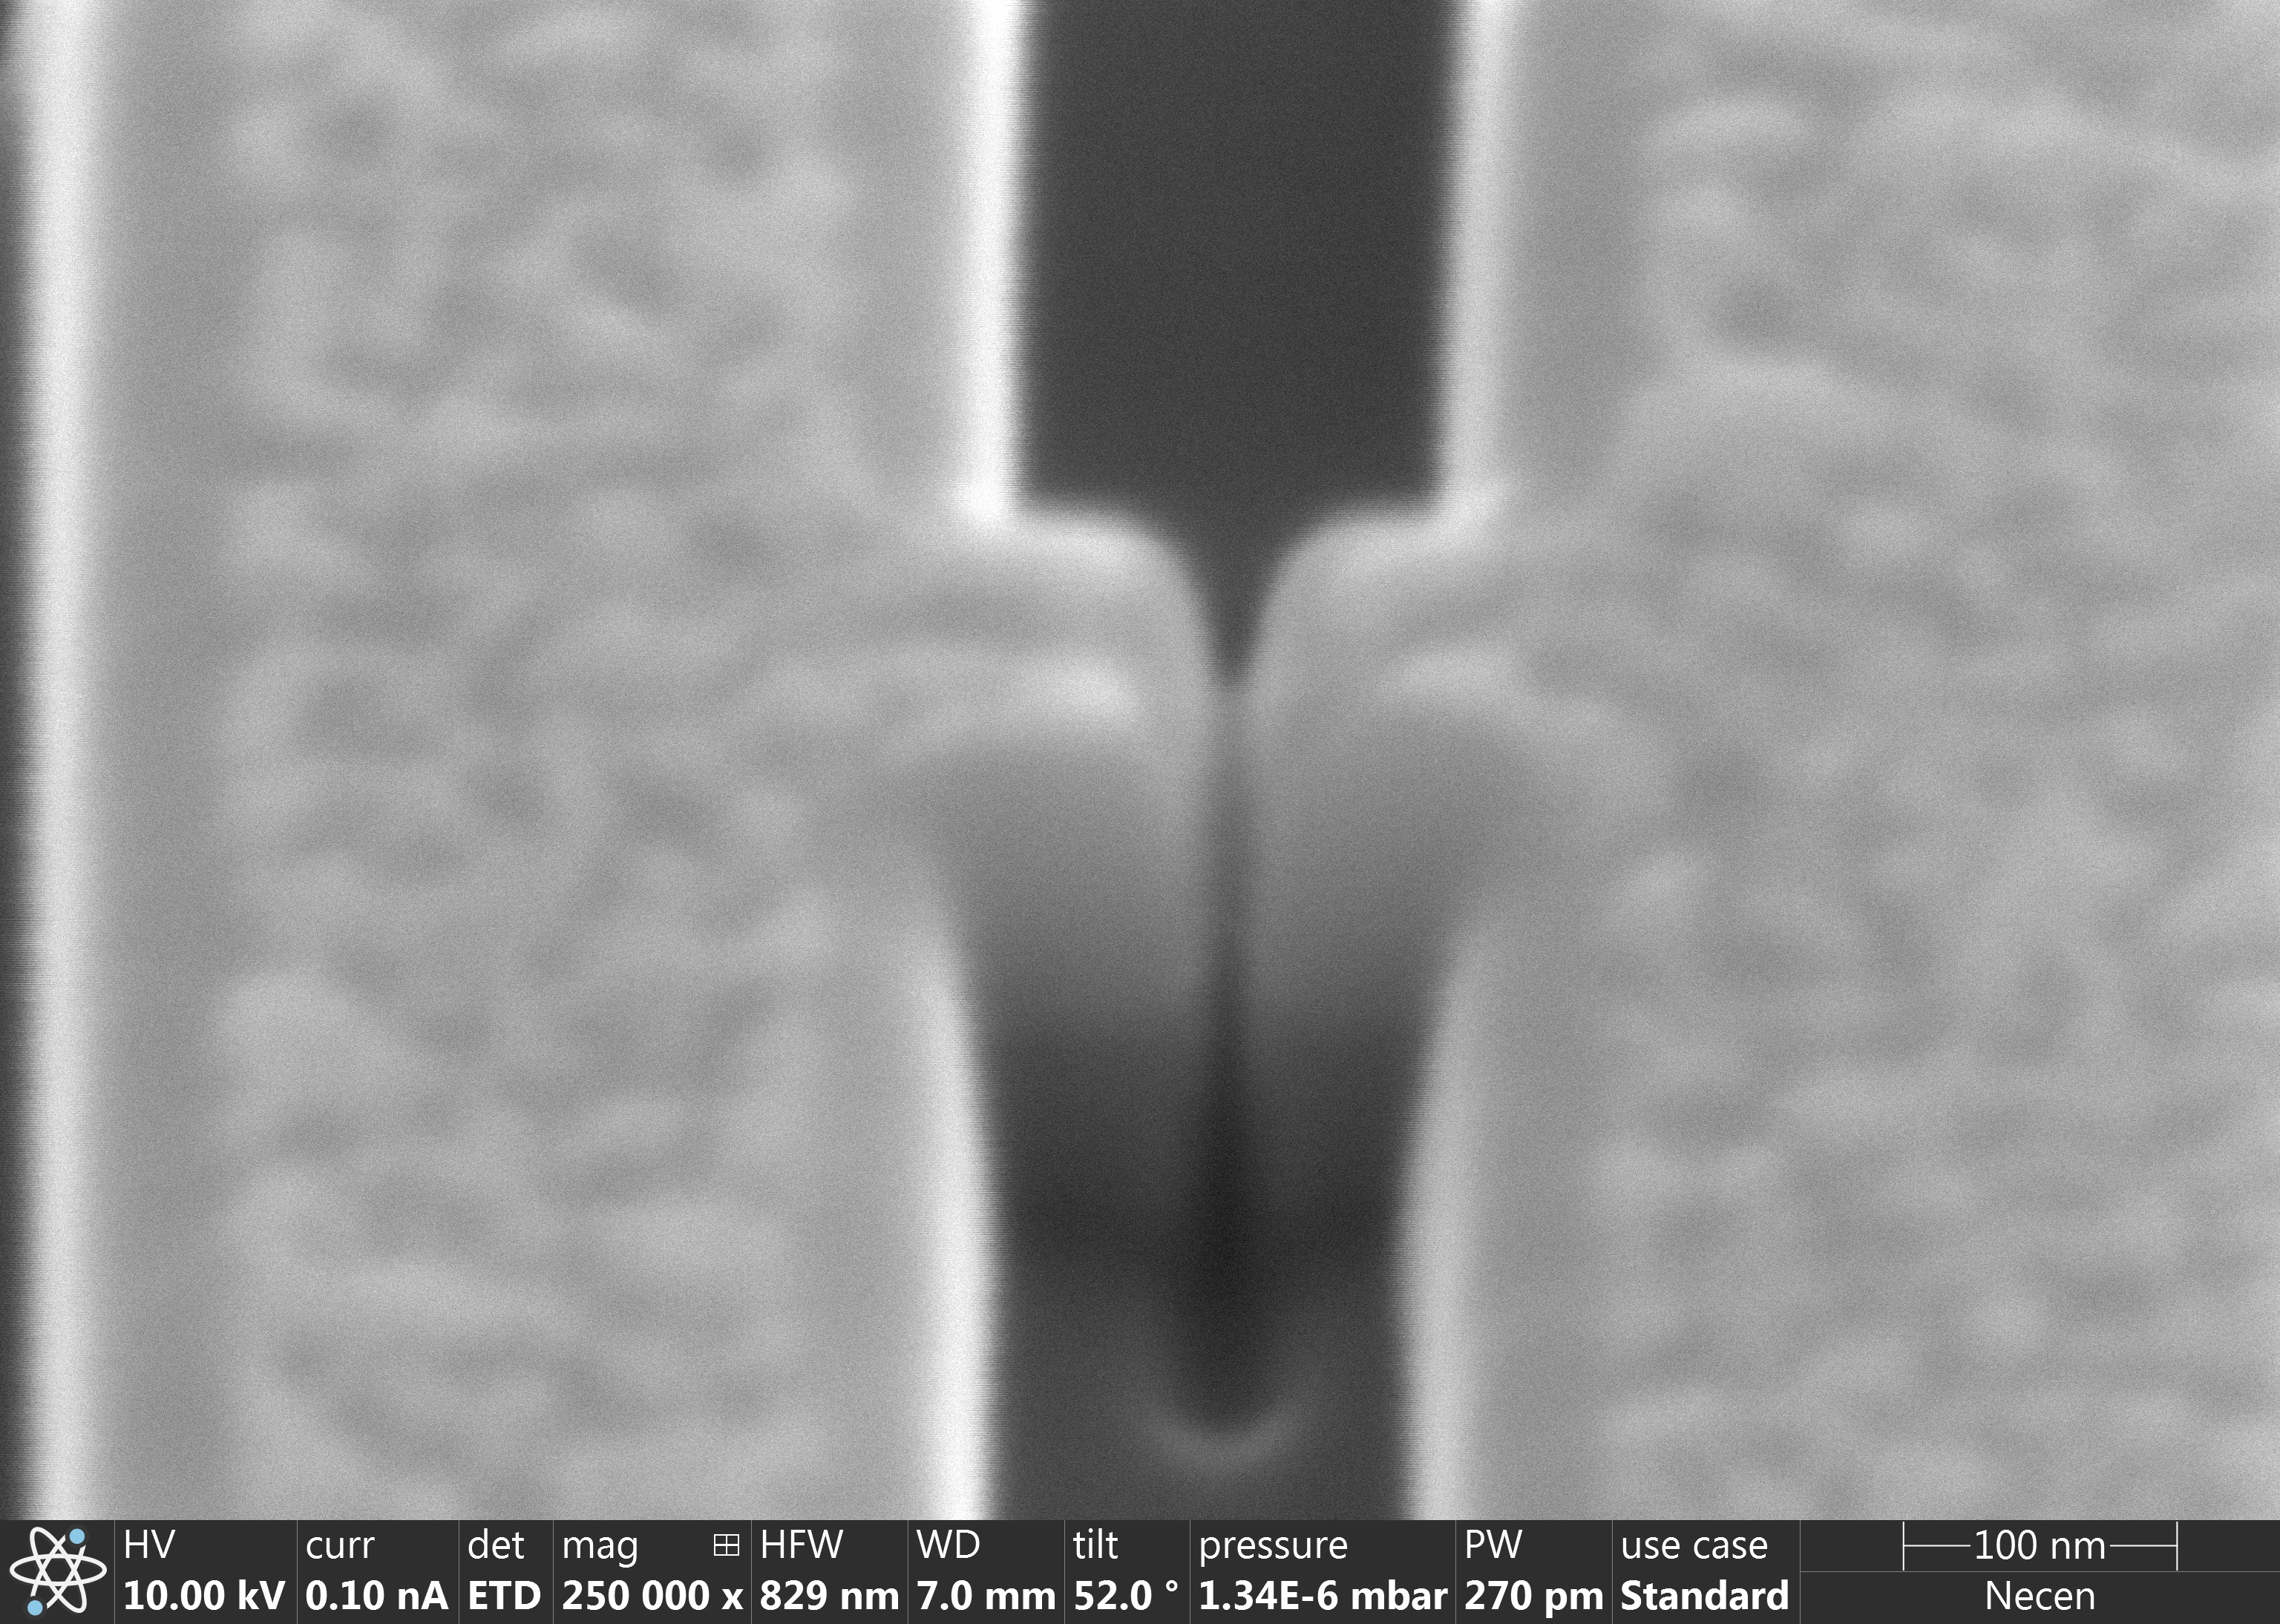
\includegraphics[width=\textwidth]{figures/samples/CP2/CP2.6B_SEM_junction.jpg}
		\subcaption{The Josephson junction under study. The width of the junction is around \qty{12}{\nano\meter}.}
	\end{subfigure}
	\hfill
	\begin{subfigure}[t]{0.3\textwidth}
		\centering
		\includegraphics[width=\textwidth]{figures/samples/CP2/CP2.6B_SEM_SQUID.jpg}
		\subcaption{The dc-SQUID, its inner and outer diameter are \qty{1.0}{\micro\meter} and \qty{1.4}{\micro\meter} respectively. The width of the junctions is \qty{22}{\nano\meter}.}
	\end{subfigure}

	% TODO: fix values.
	\caption{SEM images of sample CP2.6B.}
	\label{fig:CP2.6B-SEM-images}
\end{figure}